%=========================================================

% Here you can choose to compile with or without solutions.
% However, this definition is ignored if you use any
% command from the `Makefile`.
\providecommand{\withSol}{\iftrue}

%=========================================================

\documentclass
[twoside,german,colorbacktitle,accentcolor=tud9c]
{tudexercise}

\usepackage[T1]{fontenc}
\usepackage[utf8]{inputenc}
\usepackage[ngerman]{babel}
\usepackage{amstext}
\usepackage{amsmath}
\usepackage{graphicx}
%\usepackage{setspace}
\usepackage{multicol}
\usepackage{mathtools}
\usepackage{dsfont}
\usepackage{units}
%\usepackage{subfigure}
\usepackage{color}
\usepackage{booktabs}
\usepackage{fancyref}
\usepackage{gensymb}
\usepackage{tikz}
\usetikzlibrary{shapes.misc} 
\usepackage[verbose]{placeins}%Floatbarrier
\tikzset{root/.style={align=center,draw=none},level 2/.style={align=center,left=1.5cm}}


%=========================================================


\setcounter{section}{5}
%=========================================================

\newcommand{\grp}{F}

%=========================================================


\begin{document}

\title{GDV 2 -- Theorie Übung \arabic{section}}
\subtitle{Sommer Semester 2019}
\subsubtitle{Übungsgruppe \grp{}}

\maketitle

%=========================================================



\begin{examheader}
	\textmb{GDV 2 - Theorie Übung \arabic{section} | Gruppe \grp{}}\\
	\begin{tabular}{l l l l l}
		Moritz Fuchs	& Alexander Jäger	& Amon Ditzinger	& John Kalkhof	\\
	\end{tabular}
\end{examheader} 


%=========================================================
% Anpassung an Aufgabenstellung
\renewcommand\thesubsection{Aufgabe \arabic{subsection}}
\renewcommand\thesubsubsection{\alph{subsubsection})}

%=========================================================
\FloatBarrier
\newif\ifvimbug
\vimbugfalse

\ifvimbug
\begin{document}
\fi


\subsection{Marching Cubes (3 Punkte)}
\subsubsection{1 Punkt}
Alle blauen Punkte sind innen, alle grünen außen. Die roten Linien sind die eindeutigen Kanten / Zellen und die Zellen mit den orangenen und gelben Linien sind uneindeutig. Hierbei kann entweder orange oder gelb gewählt werden. \\
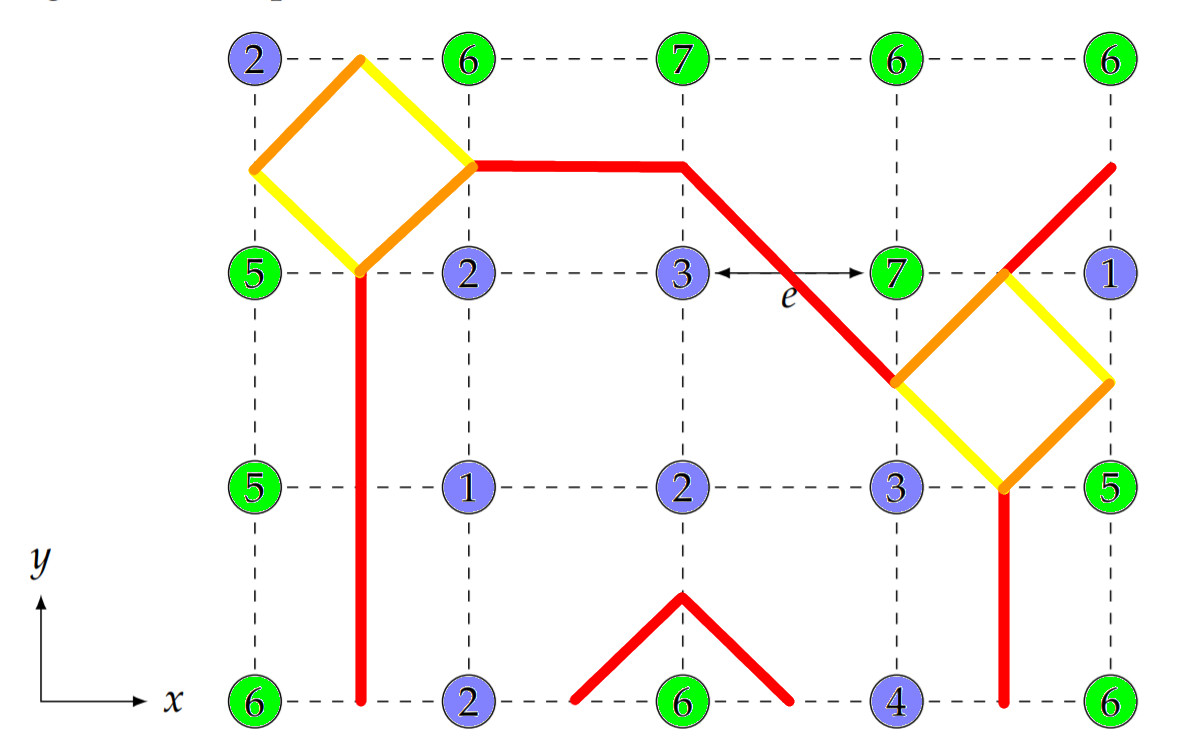
\includegraphics[width=(\textwidth/2)]{51a.jpg} 
\subsubsection{1 Punkt}
\subsubsection{1 Punkt}
\newif\ifvimbug
\vimbugfalse

\ifvimbug
\begin{document}
\fi


\subsection{Emissions-Absorptions Model (6 Punkte)}
\begin{tabular}{lcr}
  Dichtewert & q & k \\
  1 & 0.1 & 0.1 \\
  2	& 0.4 & 0.2\\
  3	& 0.9 & 0.3\\
  5	& 2.5 & 0.5\\
  6	& 3.6 & 0.6\\
  7	& 4.9 & 0.7\\
 \end{tabular}

Bilineare Interpolation über Stützpunkte R1 und R2:\\
\\
$k(R_1) = \frac{4-3.5}{4-3} * 0.7 + \frac{3.5-3}{4-3} * 0.1 = 0.35 + 0.05 = 0.4$\\
$q(R_1) = 0.5 * 4.9 + 0.5 * 0.1 = 2.45 + 0.05 = 2.5$\\
$k(R_2) = 0.5 * 0.6 + 0.5 * 0.6 = 0.6$\\
$q(R_2) = 0.5 * 3.6 + 0.5 * 3.6 = 3.6$\\
$k(s_1) = \frac{3-2.75}{3-2} * k(R_1) + \frac{2.75 - 2}{3-2} * k(R_2) = 0.25 * 0.4 + 0.75 * 0.6 = 0.55$\\
$q(s_1) = 0.25 * 2.5 + 0.75 * 3.6 = 3.325$\\
\\
Also ergibt sich $I(s_{1})$ folgenderma"sen, wobei man das Delta X einfach an der X-achse ablesen kann(Delta x = 0.5):\\
\\
$I(s_1) = I(s_0) * e^{-k(s_1)*\Delta x} + q(s_1)*\Delta x = 0.5 * \frac{1}{e^{0.55*0.5}} + 3.325 * 0.5 = 2.042$\\
\\
Nach dem selben Prinzip wird der Rest auch berechnet.\\
\\
$q(R_3) = \frac{2-1.5}{2-1} * 0.4 + \frac{1.5-1}{2-1} * 0.9 = 0.2 + 0.45 = 0.65$\\
$k(R_3) = 0.5 * 0.2 + 0.5 * 0.3 = 0.1 + 0.15 = 0.25$\\
$q(R_4) = 0.5 * 3.6 + 0.5 * 4.9 = 4.25$\\
$k(R_4) = 0.5 * 0.6 + 0.5 * 0.7 = 0.65$\\
$k(s_2) = \frac{1}{4} * 0.25 + \frac{3}{4} * 0.65 = 0.55$\\
$q(s_2) = 0.25 * 0.65 + 0.75 * 4.25 = 3.35$\\
$I(s_2) = 2.042 * \frac{1}{e^{0.55*2}} + 3.35 * 2 = 7.379$\\
\\
Und für s3 braucht man den ersten Schritt nicht, da sich der Punkt auf der y-Achse zwischen zwei Gitterpunkten befindet:\\
\\
$k(s_3) = \frac{1}{4} * 0.5 + \frac{3}{4} * 0.2 = 0.275$\\
$q(s_3) = 0.25 * 2.5 + 0.75 * 0.4 = 0.925$\\
$I(s_3) = 7.779 * \frac{1}{e^{0.275*1.5}} + 0.925 * 1.5 = 6.272$\\
\\
Und weil es so schön war nocheinmal das ganze für $\hat{s}$....\\
\\
$q(R_5) = \frac{1}{2} * 0.9 + \frac{1}{2} * 2.5 = 1.7$\\
$k(R_5) = 0.5 * 0.3 + 0.5 * 0.5 = 0.4$\\
$q(R_6) = 0.5 * 4.9 + 0.5 * 0.1 = 2.5$\\
$k(R_6) = 0.5 * 0.7 + 0.5 * 0.1 = 0.4$\\
$k(\hat{s_1}) = \frac{1}{2} * 0.4 + \frac{1}{2} * 0.4 = 0.4$\\
$q(\hat{s_1}) = 0.5 * 1.7 + 0.5 * 2.5 = 2.1$\\
$I(\hat{s_1}) = 0.5 * \frac{1}{e^{0.4*0.5}} + 2.1 * 0.5 = 1.459$\\
\\
Für $\hat{s2}$:\\
\\
$q(R_7) = \frac{1}{2} * 0.1 + \frac{1}{2} * 0.4 = 0.25$\\
$k(R_7) = 0.5 * 0.1 + 0.5 * 0.2 = 0.15$\\
$q(R_8) = 0.5 * 0.4 + 0.5 * 0.9 = 0.65$\\
$k(R_8) = 0.5 * 0.2 + 0.5 * 0.3 = 0.25$\\
$k(\hat{s_2}) = \frac{1}{2} * 0.15 + \frac{1}{2} * 0.25 = 0.2$\\
$q(\hat{s_2}) = 0.5 * 0.25 + 0.5 * 0.65 = 0.45$\\
$I(\hat{s_2}) = 1.459 * \frac{1}{e^{0.2 * 2}} + 0.45 * 2 = 1.878$\\
\\
Und $\hat{s3}$:\\
\\
$k(\hat{s_3}) = 0.5$\\
$q(\hat{s_3}) = 0.5 * 2.5 + 0.5 * 2.5 = 2.5$\\
$I(\hat{s_3}) = 1.878 * \frac{1}{e^{0.5*1.5}} + 2.5 * 1.5 = 4.637$\\

\newif\ifvimbug
\vimbugfalse

\ifvimbug
\begin{document}
\fi


\subsection{Bernstein-Bézier-Tensorprodukte (7 Punkte)}
\subsubsection{3 Punkte}
Wir wenden de Casteljau an mit $v=\frac{3}{4}$ und $\lambda= \frac{1}{4}$:\\
\begin{tikzpicture}[grow=left,
level 1/.style={sibling distance=15mm},edge from parent/.style={-,draw},>=latex, level 3/.style={edge from child/.style={->,draw},sibling distance=15mm}]

\node[root] {$\begin{pmatrix}-2.125\\ 2.5625\\5.4375\end{pmatrix}$}
     child {node[level 2] (c1) {$\begin{pmatrix}-1\\2\\3\end{pmatrix}$}
           child {node[level 2] (c11) {$\begin{pmatrix}-1\\2\\0\end{pmatrix}$}}
       child {node[level 2] (c21) {}}
       }
 child {node[level 2] (c2) {$\begin{pmatrix}-2.5\\2.75\\6.25\end{pmatrix}$}
	child {node[level 2] (c21) {$\begin{pmatrix}-1\\2\\4\end{pmatrix}$}}
       child {node[level 2] (c22) {$\begin{pmatrix}-3\\3\\7\end{pmatrix}$}}
       };
       \draw[-, draw] (c21) -- (c2);
\end{tikzpicture}\\

\begin{tikzpicture}[grow=left,
level 1/.style={sibling distance=15mm},edge from parent/.style={-,draw},>=latex, level 3/.style={edge from child/.style={->,draw},sibling distance=15mm}]

\node[root] {$\begin{pmatrix}3\\3.4375\\4.875 \end{pmatrix}$}
     child {node[level 2] (c1) {$\begin{pmatrix}3\\2.5\\3 \end{pmatrix}$}
           child {node[level 2] (c11) {$\begin{pmatrix}3\\1\\0\end{pmatrix}$}}
       child {node[level 2] (c21) {}}
       }
 child {node[level 2] (c2) {$\begin{pmatrix}3\\3.75\\5.5 \end{pmatrix}$}
	child {node[level 2] (c21) {$\begin{pmatrix}3\\3\\4\end{pmatrix}$}}
       child {node[level 2] (c22) {$\begin{pmatrix}3\\4\\6\end{pmatrix}$}}
       };
       \draw[-, draw] (c21) -- (c2);
\end{tikzpicture}\\

\begin{tikzpicture}[grow=left,
level 1/.style={sibling distance=15mm},edge from parent/.style={-,draw},>=latex, level 3/.style={edge from child/.style={->,draw},sibling distance=15mm}]

\node[root] {$\begin{pmatrix}6.5\\1.375\\6.5625 \end{pmatrix}$}
     child {node[level 2] (c1) {$\begin{pmatrix}7.25\\1.75\\3\end{pmatrix}$}
           child {node[level 2] (c11) {$\begin{pmatrix}8\\1\\0\end{pmatrix}$}}
       child {node[level 2] (c21) {}}
       }
 child {node[level 2] (c2) {$\begin{pmatrix}6.25\\1.25\\7.75\end{pmatrix}$}
	child {node[level 2] (c21) {$\begin{pmatrix}7\\2\\4\end{pmatrix}$}}
       child {node[level 2] (c22) {$\begin{pmatrix}6\\1\\9\end{pmatrix}$}}
       };
       \draw[-, draw] (c21) -- (c2);
\end{tikzpicture}\\
Wir wenden de Casteljau an mit $u=\frac{1}{4}$ und $\lambda= \frac{3}{4}$:\\
\begin{tikzpicture}[grow=left,
level 1/.style={sibling distance=15mm},edge from parent/.style={-,draw},>=latex, level 3/.style={edge from child/.style={->,draw},sibling distance=15mm}]

\node[root] {$\begin{pmatrix}0.3359375\\2.81640625\\5.296875   \end{pmatrix}$}
     child {node[level 2] (c1) {$\begin{pmatrix}-0.84375\\2.78125\\5.296875\end{pmatrix}$}
           child {node[level 2] (c11) {$\begin{pmatrix}-2.125\\ 2.5625\\5.4375\end{pmatrix}$}}
       child {node[level 2] (c21) {}}
       }
 child {node[level 2] (c2) {$\begin{pmatrix}3.875\\2.921875\\5.296875\end{pmatrix}$}
	child {node[level 2] (c21) {$\begin{pmatrix}3\\3.4375\\4.875\end{pmatrix}$}}
       child {node[level 2] (c22) {$\begin{pmatrix}6.5\\1.375\\6.5625 \end{pmatrix}$}}
       };
       \draw[-, draw] (c21) -- (c2);
\end{tikzpicture}\\
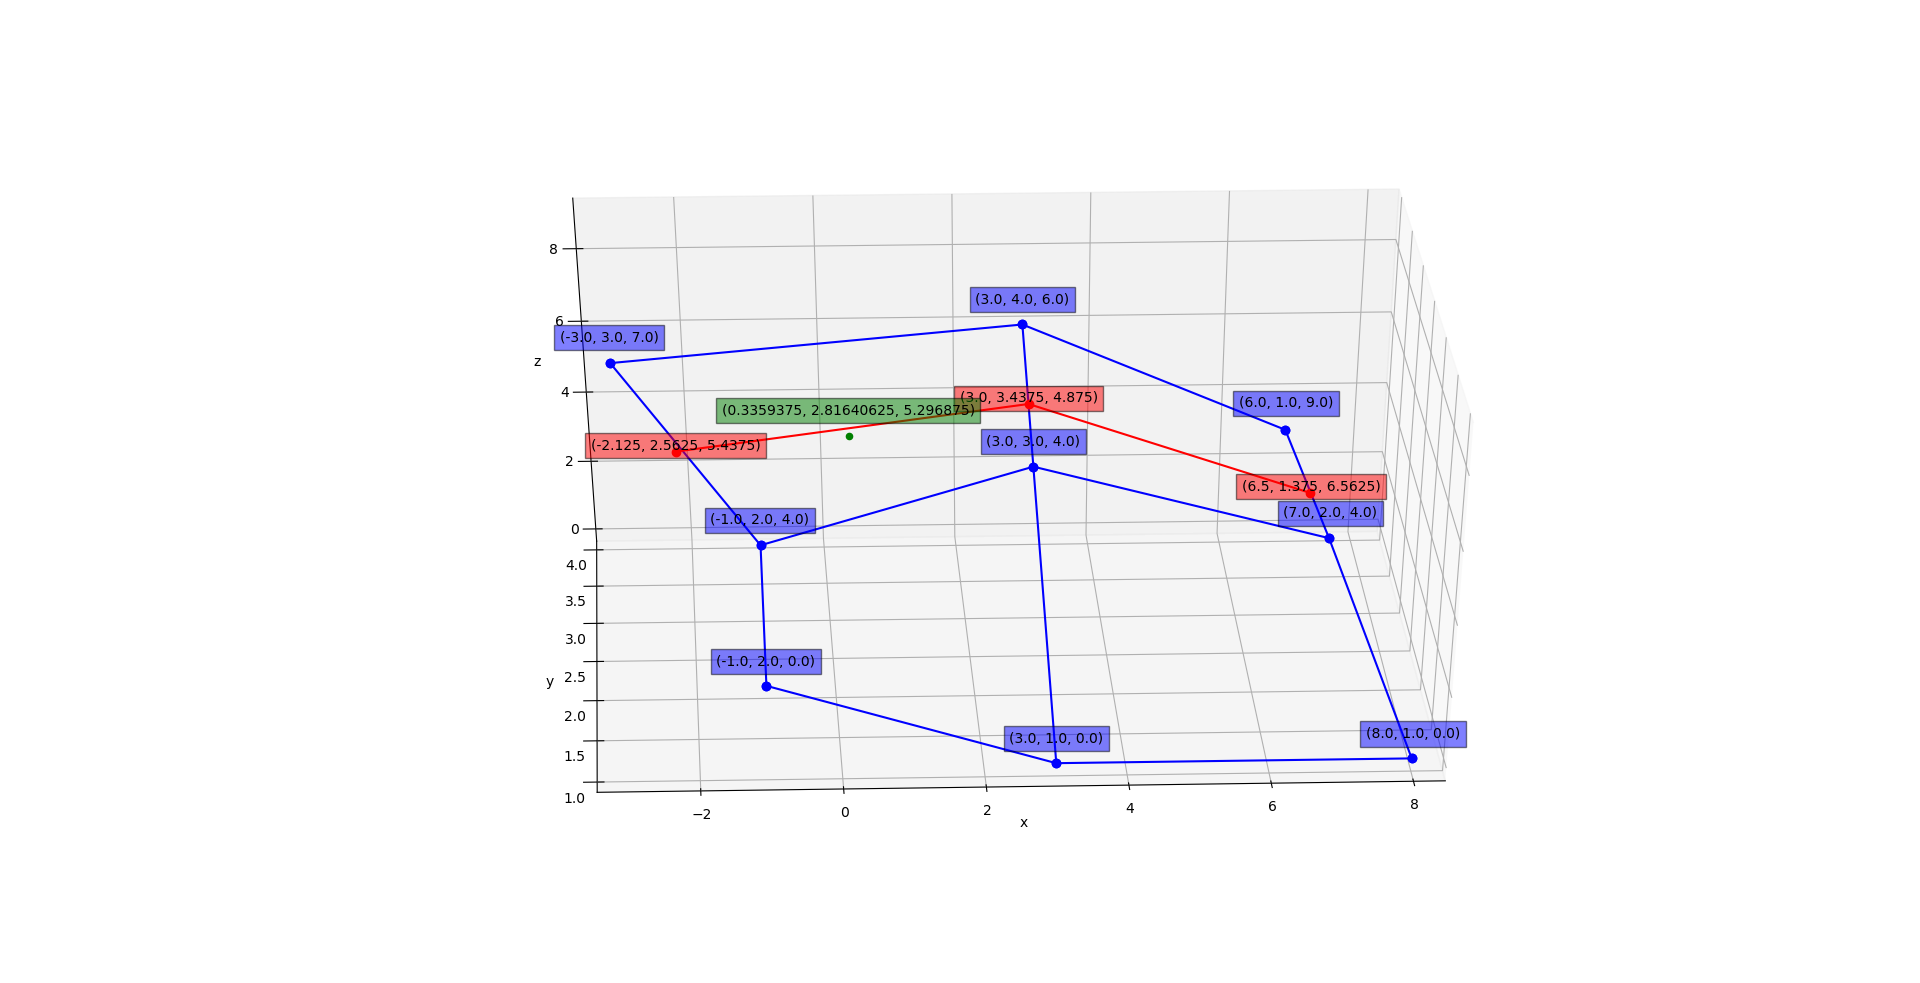
\includegraphics[width=0.9\textwidth]{2_a.png}
\subsubsection{2 Punkte}
hierzu bestimmen wir die kontrollpunkte an den Intervallsgrenzen, wie in Aufgabeteil a. in der grafik sind ist die Neue untereilung eingezeichnet.\\ 
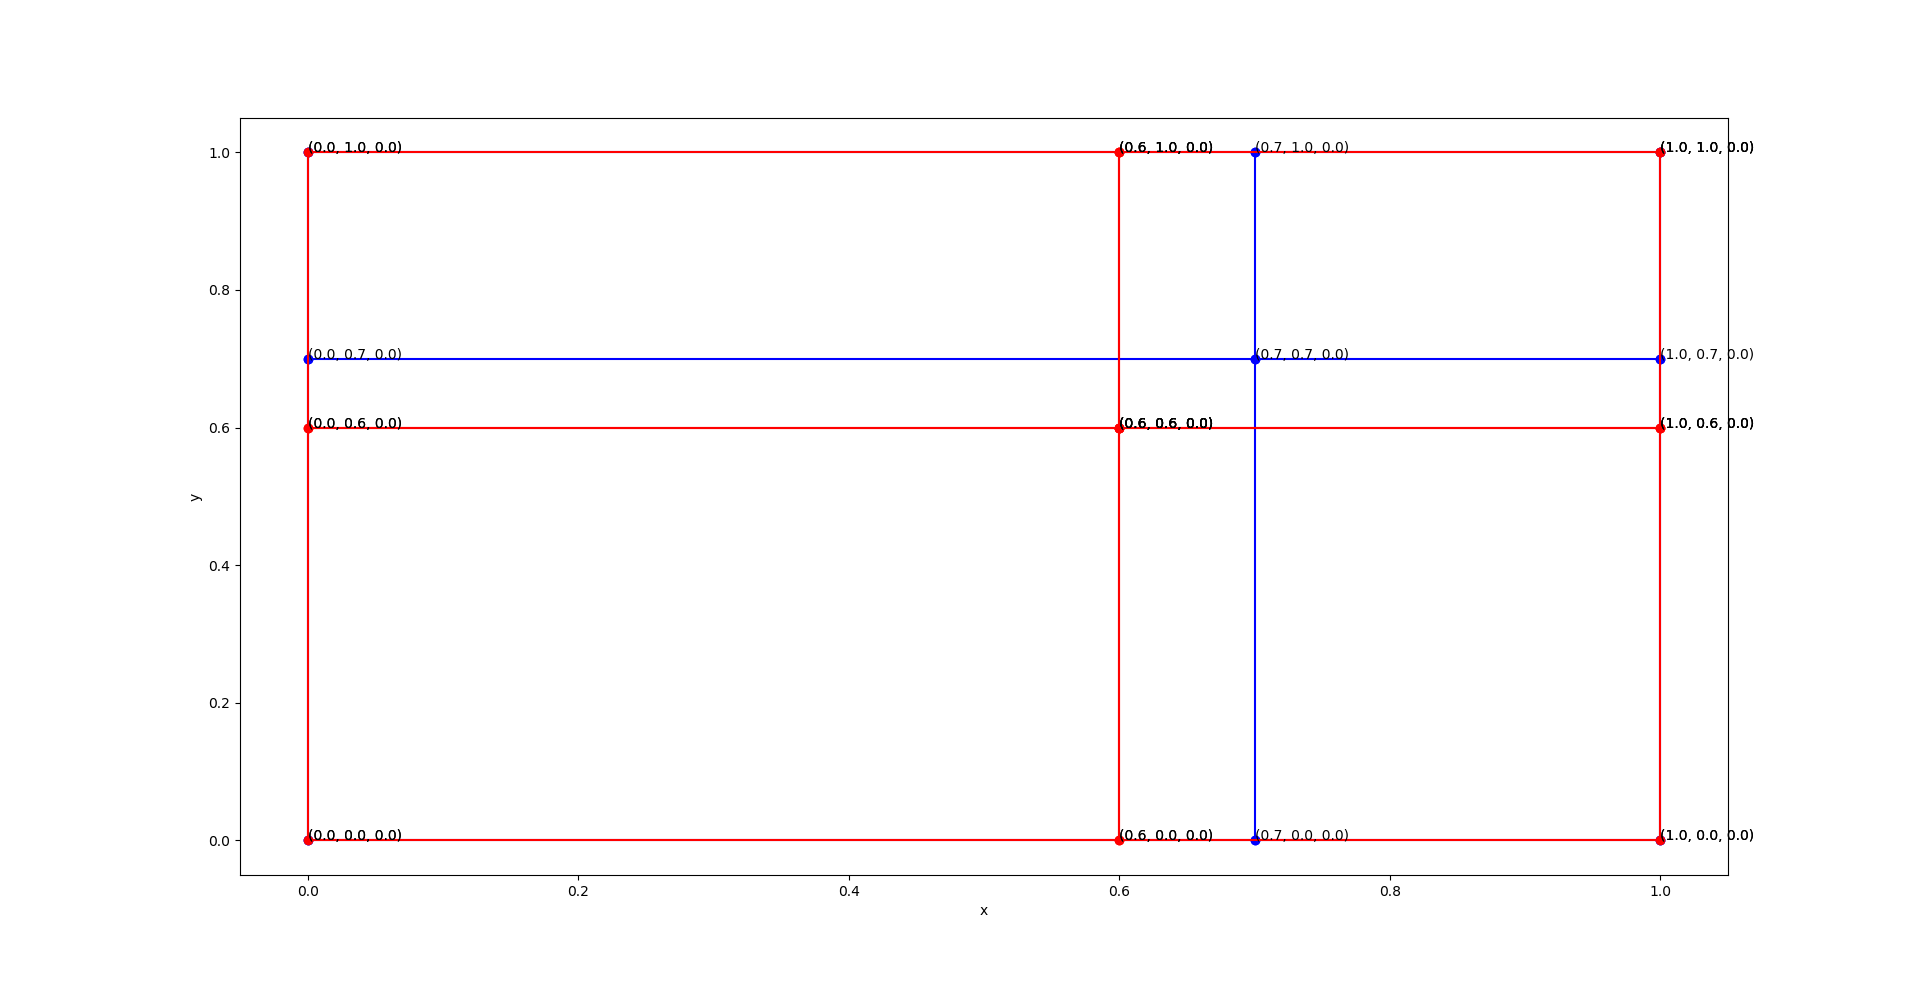
\includegraphics[width=0.9\textwidth]{2_b.png}
\subsubsection{2 Punkte}
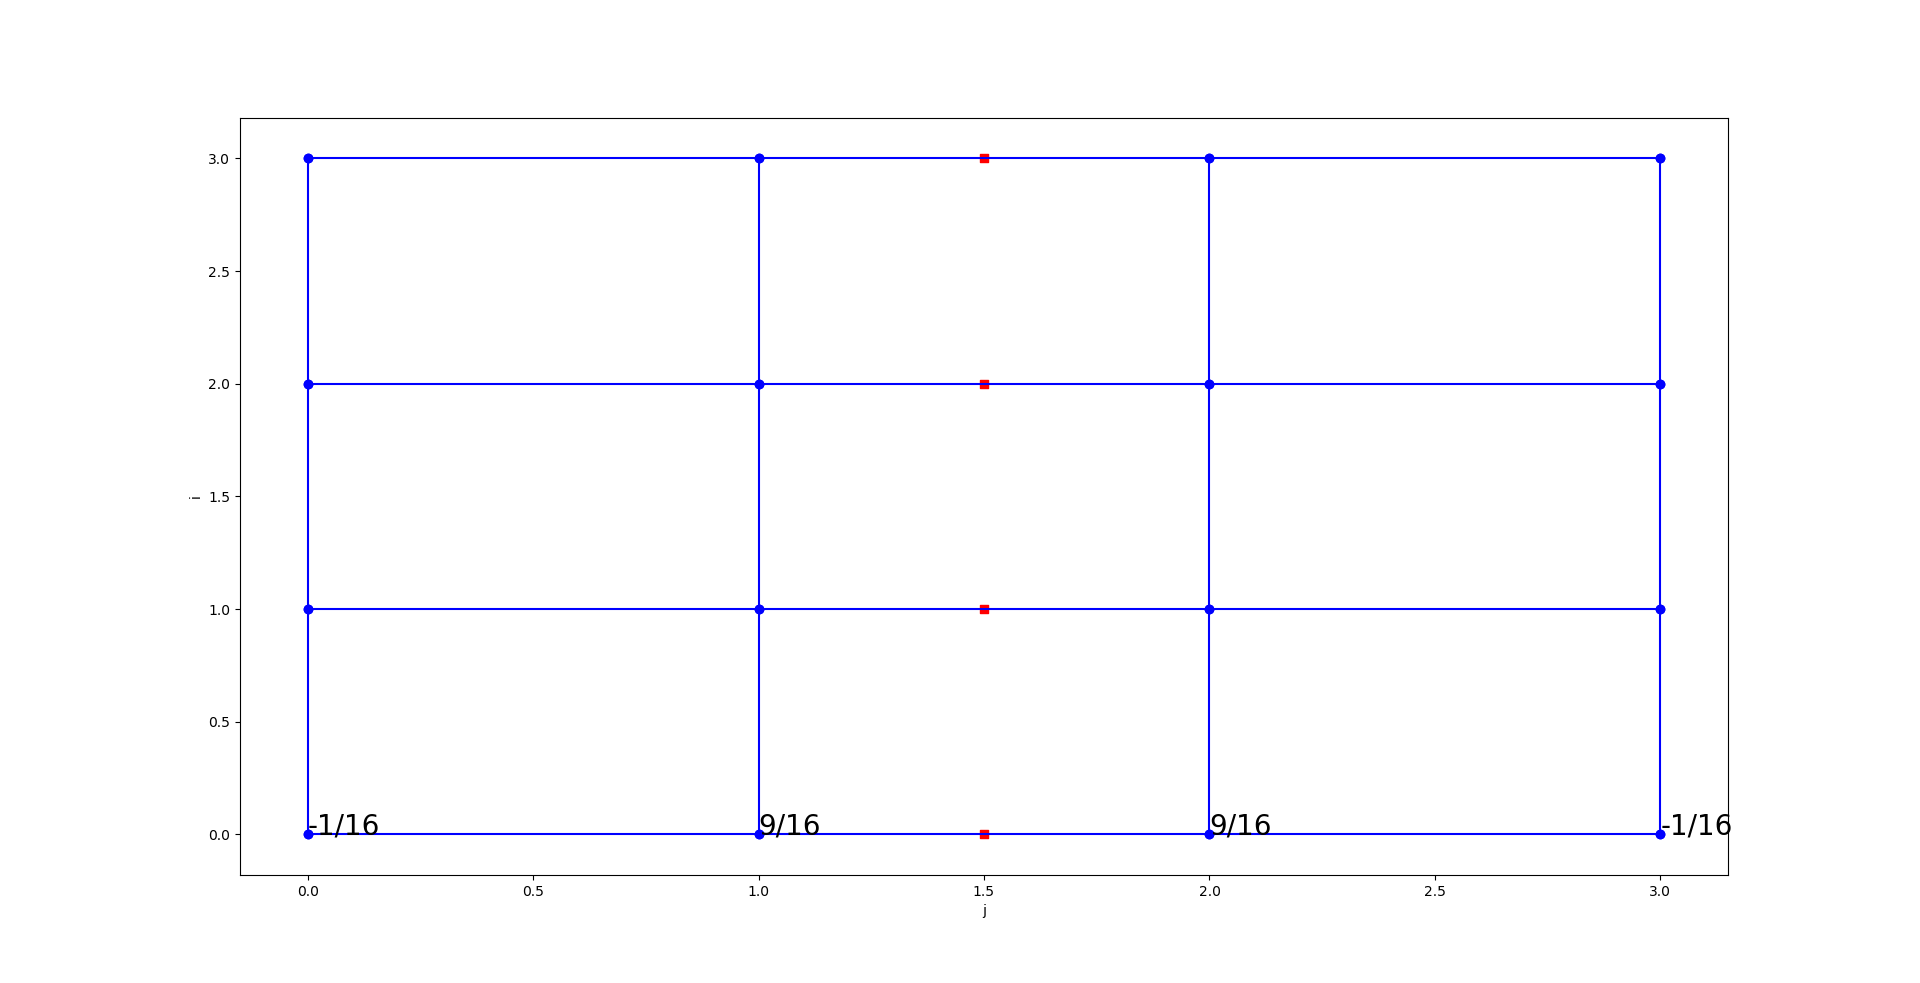
\includegraphics[width=0.5\textwidth]{2_c_P1.png}\\
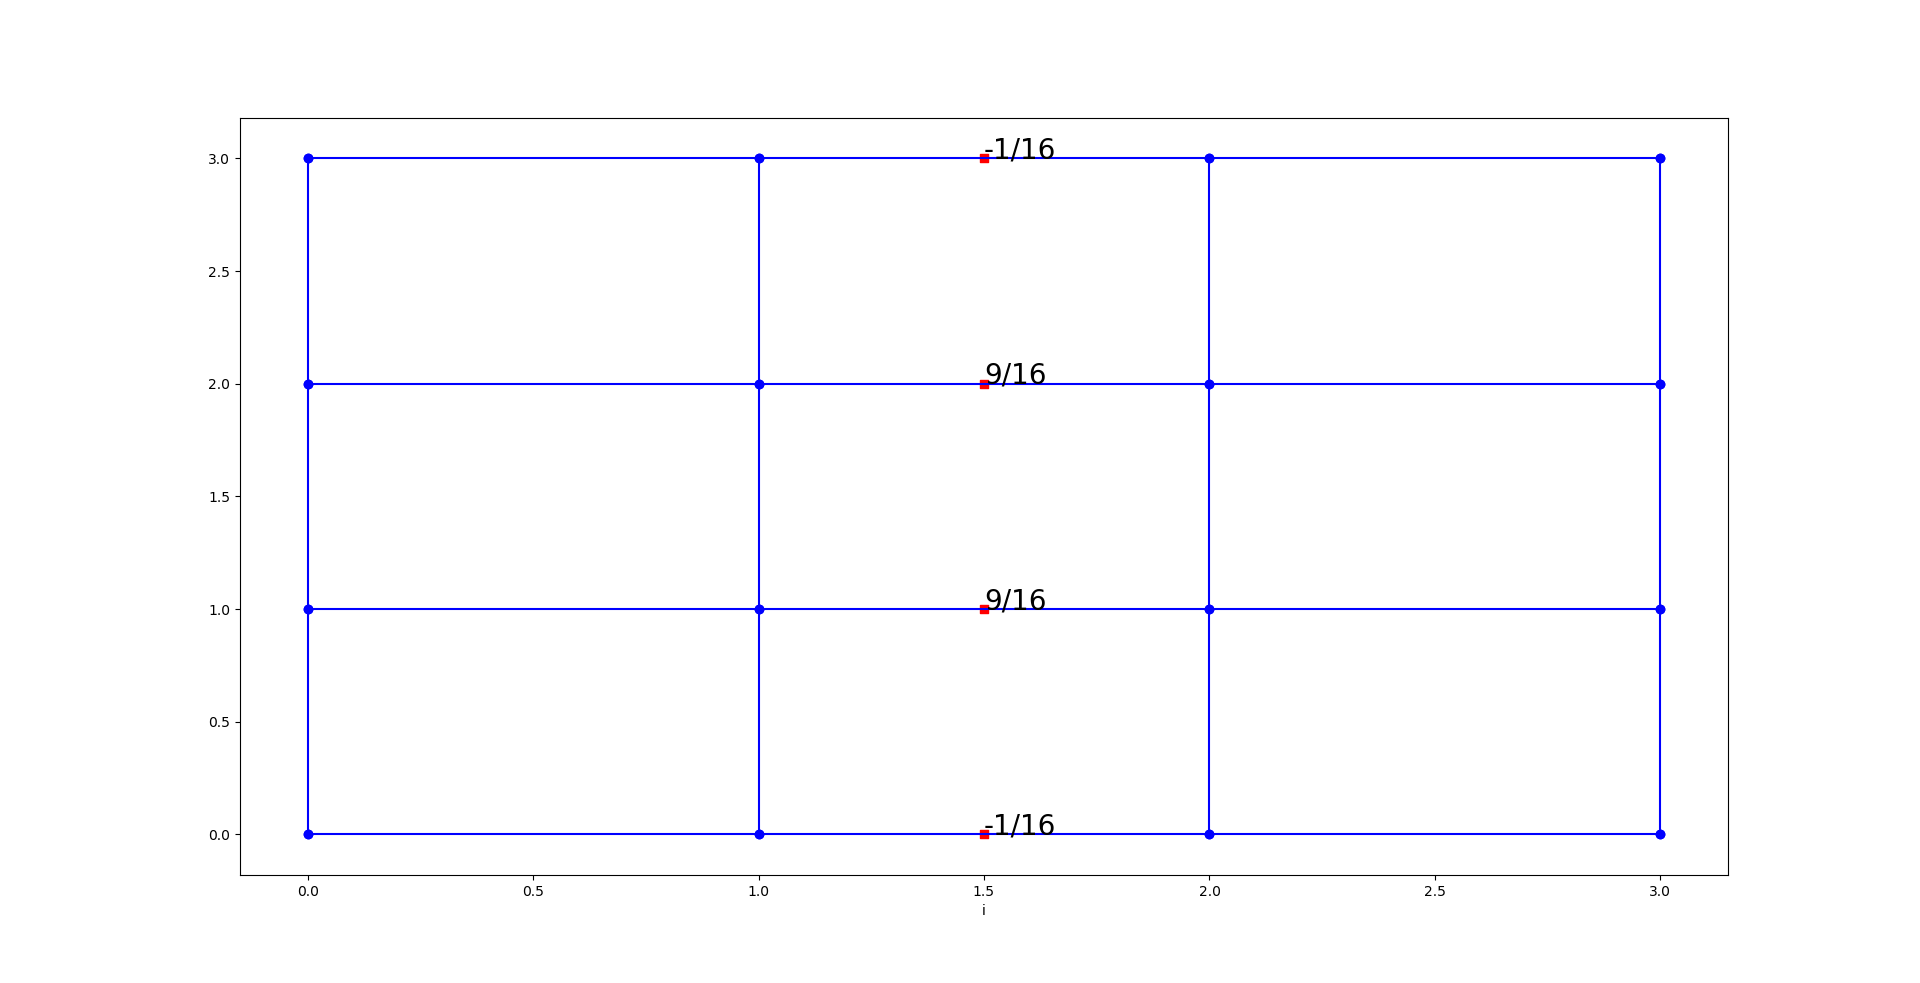
\includegraphics[width=0.5\textwidth]{2_c_P2.png}\\
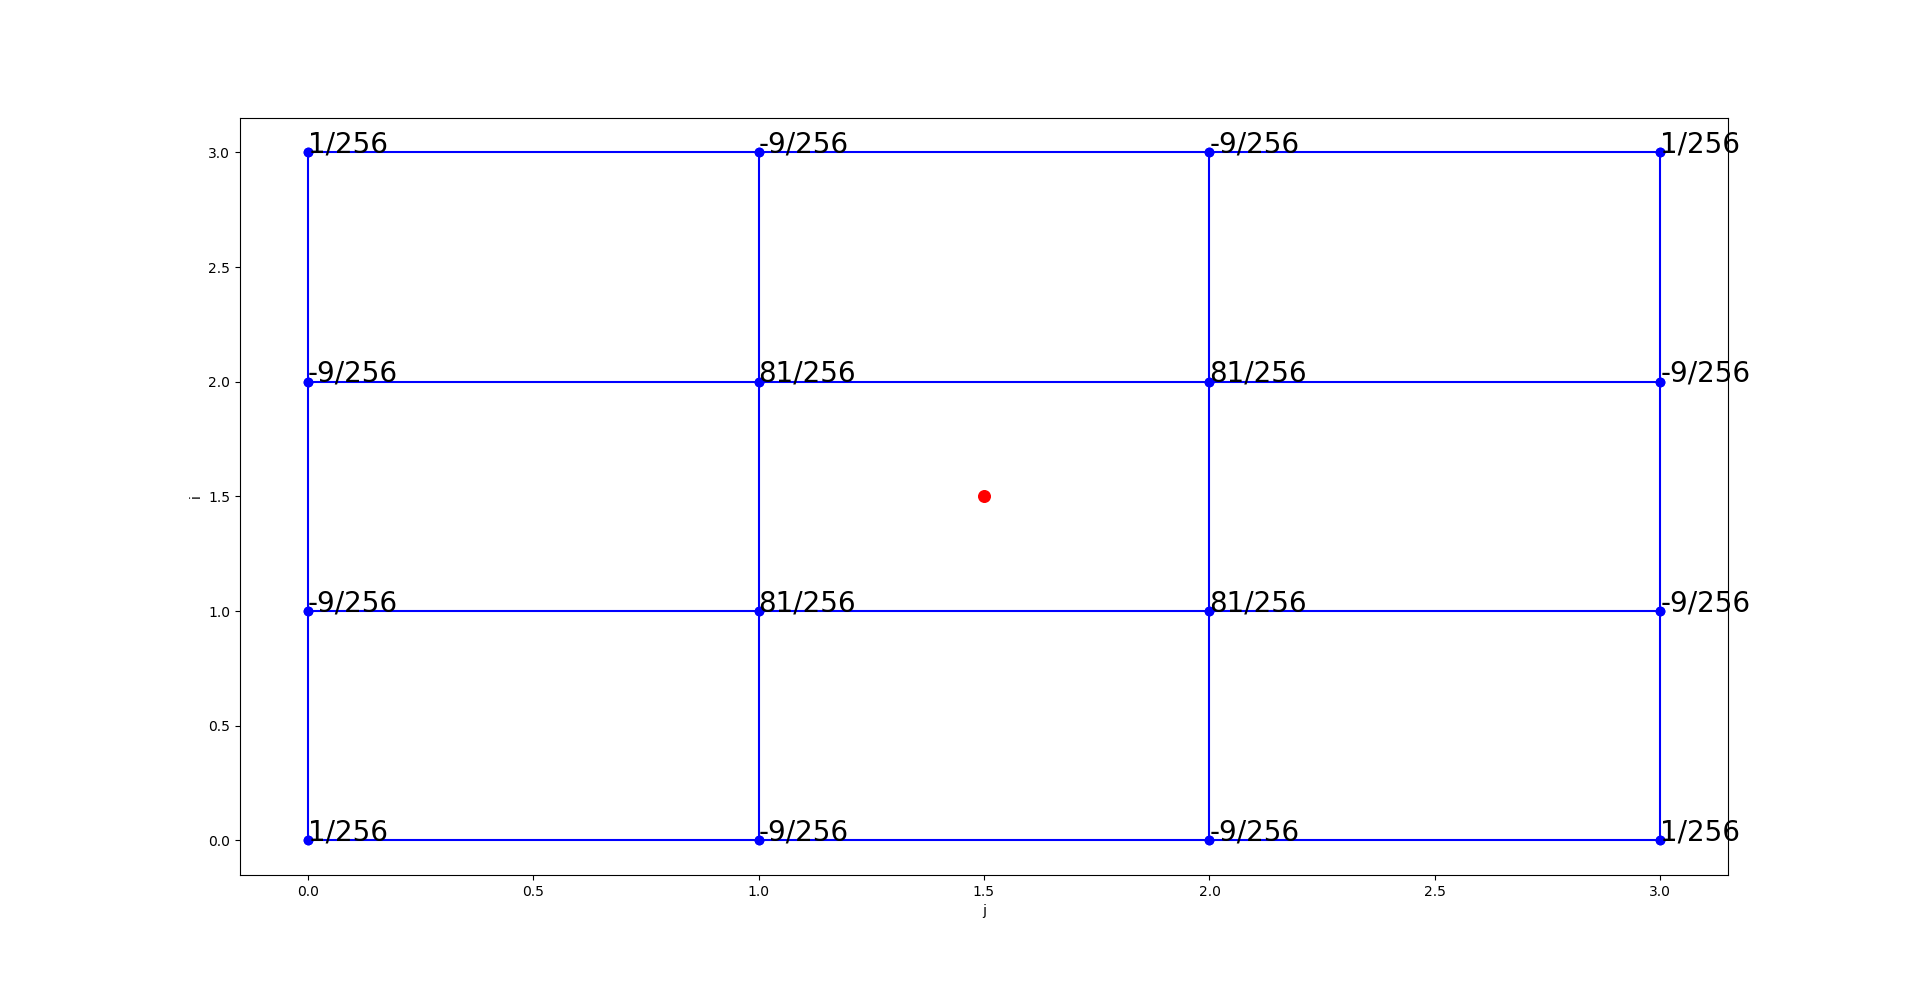
\includegraphics[width=0.5\textwidth]{2_c_P3.png}
\newif\ifvimbug
\vimbugfalse

\ifvimbug
\begin{document}
\fi


\subsection{Splines auf Triangulierungen (5 Punkte)}



%=========================================================

\end{document}
